\chapter{Lektion 2}
\section{Kapitel 5}
\subsection{The law of demand}
\textbf{Loven om efterspørgsel} er det der siger folk gør mindre af det de vil når prisen stiger. 

Man opvejer stadig fordele og ulemper, og man man vil ikke overstige sin reservationspris. Reservationsprisen er der hvor fordele og ulemper går i 0. 

\subsubsection{The origins of demmand}
Reservationsprisen bestemmes blandt andet ud fra ens præferencer. En Justin fan vil give mange penge for et album mens andre ikke ville. Ens præferencer kan stamme fra landet, familien eller skolen du er vokset op i/ved. Det kan også afgøres af andre ting i omgivelserne, fx en populær film om dinosauer vil dinosauerlegetøj stige. Ens forbrug påvirkes også af venner og man gerne vil ses forbruge på det "bedste"(heller flammen i chinabox).

\subsubsection{Needs versus wants}
Ved efterspørgsel kan man skille behov og ønsker ad. Når man fået mad, tag over hoved og det nødvendige tøj så vi er sunde og raske 

\subsection{Translating wants into demand}
Vi har ikke ubegrænsede resourcer og skal derfor fordele dem på de vigtigste ting, og det der giver mest nytte i alt. 

\subsubsection{Measuring wants: the concept of utility}
Nytte er et koncept der repræsentere folks tilfredshed ved deres forbrug. Det at folk prøver at maksimere tilfredsheden, kaldes for nytte maksimering. Hvis at købe en is bringer dig nytte, er det ikke sikkert at købe 10 is vil bringe dig 10 gange så meget lykke, ikke engang hvis de var gratis. 
%

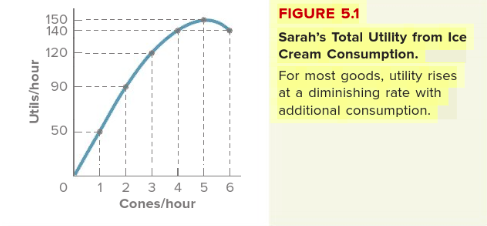
\includegraphics[scale=0.8]{Afsnit/Lektion2/Sarahkoberis.png}

Det ses her at \textbf{marginal nytten} falder fra 50 til 40 til 30 osv, indtil den tilsidst er negativ. Når marginanytten er negativ vil den \textbf{totale nytte falde}. I dette tilfælde vil fordelene overskyde ulemperne til den 5 is, og derfor vil hun købe indtil den 5. Loven om faldende marginalnytte er den lov der beskriver at bare fordi du får dobbelt så meget af noget, bliver du ikke dobbelt så glad. Der er selvfølgelig undtagelser. 

\subsubsection{Allocating a fixed income between two goods}
Det er sjældent man kun skal vurdere nytten for en ting. Hvis man har en bestemt mængde penge der kan bruges på to forskellige produkter skal man vurdere hvordan man får mest mulig lykke ud af det. Ud fra loven om faldende marginalnytte ville det ikke give mening at bruge alle pengene på en af tingene, men fordele dem på de to produkter. Når man vælger den kombination der giver den højeste totale nytte har man opnået \textbf{optimal kombination af varer}. Det kan bestemmes ved at finde der hvor nytten ift penge er det samme for alle varerne, da det her ikke er muligt at hæve den totale nytte. 

\subsection{The rational spending rule}
\begin{defn}\textbf{The Rational Spending Rule} %Ny definition
\newline
Forbrug burde fordeles blandt varerne sådan at marginal nytten per kr. er den samme for hver varer. 
\end{defn}

\begin{itemize}
    \item $MU_C$ - marginal nytte af chokolade i utils per pint
    \item $P_C$ - Pris for chokolade i kr per pint
    \item $\frac{MU_C}{P_C}$ - Marginal nytte per kr i util per kr
    \item Det samme med V for vanilje
\end{itemize}
Så vil man maksimere den totale nytte ved
\begin{align*}
    \frac{MU_C}{P_C} = \frac{MU_V}{P_V}
\end{align*}
Hvis højresiden er større end vestresiden skal man købe mere af højresiden. Det er selvfølgelig ikke alting man kan bruge denne teori på, fx tv. Man må stadig ikke tage gennemsnittet og gå ud fra som ved alt mulig andet i økonomi. 

\subsubsection{Income and substitution effects revisited}
Substitutionseffekten: hvis prisen stiger på en varer skifter man til substitutionen, og dens efterspørgselskurve flyttes til højre. Indkomsteffkten: Hvis indkomsten falder flyttes efterspørgselskurven for normale varer til venstre, folk har ikke råd til lige så meget. 

Hvis prisen på noget stiger vil marginal nytten falde og man vil derfor skulle bruge flere penge på en anden varer istedet for den med prisstigningen, for at opnå maksimal total nytte. 
\subsubsection{Applying the rational spending rule}
Når man ser en stigning i priser og folk skifter til en substitut varer er det fordi at den reel pris stiger. Altså stiger prisen ift andre priser. Det betyder at bare fordi den nominelle pris stiger betyder det ikke at folk skifter, hvis priserne på alt andet også stiger. 

\textbf{The importance of income differences}
Jo flere penge man har jo mere villig er man til at betale mere for ting, da det ikke er en lige så står del af ens indkomst som hvis man ikke tjente meget. 

\subsection{Individual and market demand curves}
Hvis man kender hvert individs efterspørgsel efter en varer, kan man lave en efterspørgselskurve for varen over hele markedet. Det gør man ved \textbf{horisontalt addition}. Hvis der kun er to købere på is-markedet, Sarah og Tom. Sarah efterspørger 2 is til prisen 4kr og Tom efterspørger 3 is til prisen 4kr, så er den samlede efterspørgsel på is-markedet 5 is til prisen 4kr. 

\subsection{Demand and consumer surplus}
\textbf{Forbrugeren overskud} er forskellen mellem prisen og forbrugerens reservationspris. Dette kan bruges til at beregne det totale overskud for alle forbrugere på markedet. 

\subsubsection{Calculating consumer surplus}
\begin{eks} \textbf{} %Nyt eksempel
\newline
Der er 11 købere der hver især kan købe max. 1 vare om dagen. Køber 1 har en reservationspris på 11kr, den næste 10, den næste 9 osv. Efterspørgselskurven vil være en trappe. Hvis den efterspurgtvarer kostede 6kr, ville der blive solgt 6 enheder om dagen. 5 af køberne vil have overskud og den sidste vil gå i 0. Overskudende vil være henholdsvis være 1, 2, 3, 4 og 5 kr. Det samlede overskud ville her være 15kr. 
\end{eks}

Dette kan overføres til en almindelig efterspørgsels og udbudskurve. Bare find arealet af trekanten. På billedet er overskuddet 2000 gallons/day. 

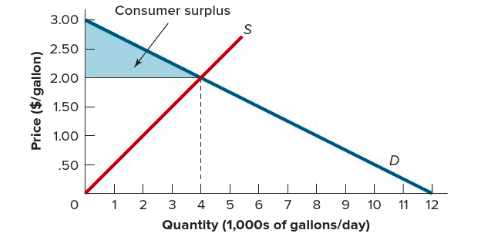
\includegraphics[scale=0.8]{Afsnit/Lektion2/Consumersurplus.png}

\section{Kapitel 6}
Over årene er produktiviteten i mange industrier steget. Industriarbejderes løn er dermed også steget, men en frisør bruger stadig lige lang tid på at klippe en person som for 30 år siden, og lønen for dem er også steget. Dette kan forklares ved at hvis frisøren ikke også fik mere i løn så kunne personen bare vælge et andet jo der gav mere i løn, men problemet er at der stadig er brug for frisører. 

\subsection{Thinking about supply: the importance of opportunity cost}
Udbudskurven laves ud fra offeromkostningerne(alternativomkostninger). Man kan sammenligne det med følgende eksampel.
\begin{eks} \textbf{} %Nyt eksempel
\newline
Harry kan enten tjene 6 kr i timen på hans arbejde eller samle dåser. Nedenfor ses mængden af dåser han kan samle.

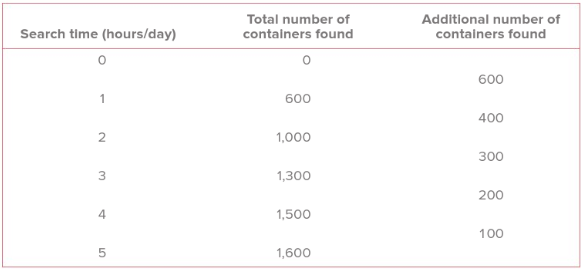
\includegraphics[scale=0.8]{Afsnit/Lektion2/Harry.png} 

Så kan den nødvendige pris for hver dåse bestemmes, for at det kan betale sig at samle dåser.
\begin{align*}
    p(\Delta Q) = 6kr\\
    \text{eks}\\
    p(400) = 6kr \Leftrightarrow p = 1.5 øre
\end{align*}
Ud fra dette kan "udbudskurven" laves.
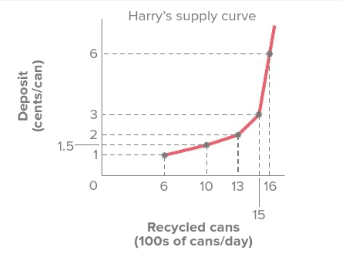
\includegraphics[scale=0.8]{Afsnit/Lektion2/Harry2.png}
\end{eks}

\subsection{Individual and market supply curves}
På samme måde som for efterspørgsel kan man bruge horisontal addition til at gå fra individuel udbud til hele markedets udbudskurve. 

Grunden til kurven har en positiv hælding kan forklares ved \textbf{the principle of increasing opportunity cost} eller \textbf{the low-hanging-fuit principle}. Det er nemmere at finde de første og det bliver dermed sværer og sværer at finde nogle "dåser". Derudover er det på grund af offeromkostningerne, jo højere prisen bliver jo flere dækker det offeromkostningerne for. Ved en lav pris, er der kun få der laver noget hvis offeromkostninger bliver dækket. Hvis vi vender tilbage til eksemplet. En for en arbejdsløs dækker at samle dåser offeromkostningerne for hvad han kunne tjene på et andet arbejde(da han ikke har et). Derimod skal prisen være en del højere før en matematikøkonom får dækket sine offeromkostninger. 

\subsection{Profit-maximizing firms in perfectly competitive markets}
\subsubsection{Profit maximization}
De fleste firmaer eksistere for \textbf{proffittens} skyld, dette er \textbf{profit-maksimerings firmaer}. Et firmas profit er forskellen på det det koster at producere varen for og det forbrugeren giver for den. 

Udbudskurven er lavet ud fra at det er profit-maksimerings firmaer der sælger en vare på et marked med fuldkommen konkurrence(perfekt konkurrence). Hvilket er markeder hvor individuelle firmaer ingen indflydelse på markedsprisen, og derfor er firmaerne \textbf{pristagere}.

\textbf{Fuldkommen konkurrence}:\\
\begin{itemize}
    \item Alle firmaer sælger samme standard produkt. Købere er altså villig til at skifte sælger for at prisen er lavere.
    \item Der er ikke nogen stor købere eller sælgere der kan styre markedet. Det består kun at små = pristagere.
    \item Man kan frit bevæge sig mellem markeder. Der er ingen bindning og alle kan skaffe det de skal bruge for at producere varen.
    \item Sælgere og købere kender alle muligheder. 
\end{itemize}
Hvede er tæt på fuldkommen konkurrence det er computermarkedet ikke, hvor microsoft styre meget, fx priser.

\subsubsection{The demand curve facing a perfectly competitive firm}
Mange af de konklussioner der kommer, kan også passer til udbud/efterspørgsel for  \textbf{ikke-fuldkommen kokurrence firmaer} som fx Microsoft.
Fordi firmaer i fuldkommen konkurrence ikke bestemmer prisen, derfor er deres individuelle udbudskurve en horisontal streg ved markedsligevægt. For hele markedet ser udbud/eftespørgselskurverne "normale" ud. 

\subsubsection{Production in the short run}
Hvordan vurdere man under fuldkommen konkurrence hvor meget man som firma skal producere. \textbf{Faktorerne for produktionen} er de input der er brugt til at producere en varer, fx arbejdskraft eller maskinleje og meget meget mere. \textbf{Kort sigt} er hvor der er nogle ting firmaet ikke kan nå at ændre, fx. de kan ikke bare nå at skifte masiker ud men de kan nå at ændre mængden af arbejdskraft. \textbf{Lang sigt} er hvor alle faktorer kan nå at ændres. 

Når inputs vokser, fx arbejdskraft vil output stiger. Dog vil det ikke stige for evigt. hvis man starter med 1 arbejder og man får 1 til gør de en stor forskel men hvis man har 100, og får 1 til gør det slet ikke det samme. 

\begin{defn}\textbf{Law of diminishing returns} %Ny definition
\newline
Når nogen faktorer i produktionen er holdt fast, vil en stigning i produktionen af en varer på et tidspunkt kræve endnu større stigning i de variable faktorer. 
\end{defn}

\textbf{Faste faktorer} er på kort sigt, dem der ikke kan nå at ændres, og de \textbf{variable faktorer} er på kort sigt dem der godt kan nå at ændres. 

\subsubsection{Some important cost concepts}
En \textbf{fast omkostning} er en omkostning der vil være der ligemeget hvor meget firmaet producere, foreksempel en husleje. Derudover er der \textbf{variable omkostninger} som varierer ift produktionen. De \textbf{totale omkostningerne} er de variable og faste omkostninger tilsammen. 
\textbf{Marginalomkostningerne} er det de totale omkostninger stiger med når man udfører én ekstra aktivitets enhed. Det er definieret som ændringen i de totale omkostning ift ændringen i output. 

\subsubsection{Choosing output to maximize profit}
Hvordan afhænger mængden af produktion af pris, løn og omkostninger af kapital. Det gælder om at maksimere profitten som er indtjening minus omkostningerne. 

\begin{eks} \textbf{} %Nyt eksempel
\newline
Man regner med at man kan sælge alle flasker til markeds prisen 0,35kr 

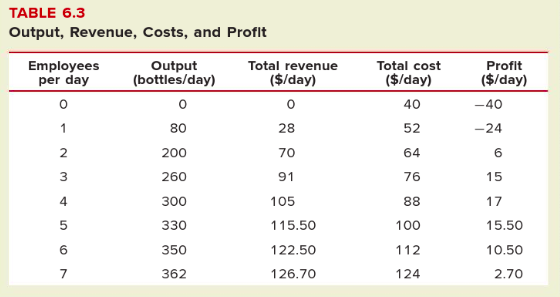
\includegraphics[scale=0.8]{Afsnit/Lektion2/maksprofit.png}

Her ses det at marginalomkostningerne er lavere end marginalfordelene indtil en produktion er på 300 flasker. Det er dermed her man opnår den maksimale profit. Et fald i lønninger vil sænke marginalomkostninger og opnå større profit. På samme måde vil en ændring i faste omkostninger også ændre profitten. 
\end{eks}

\subsubsection{A note on the firms shutdown condition}
Det er ikke altid det kan betale sig for firmaer at producere noget. Hvis prisen er så lav at indtjeningen aldrig overstiger de variable omkostninger, vil de miste mindre ved slet ikke at producere noget. Her vil de så kun have et underskud på de faste omkostninger. Hvis indtjeningen er lavere end de variable omkostninger($\frac{P}{Q}<VC$) kaldes det \textbf{kort sigtet nedluknings tilstand}.

\subsubsection{Averagee variable cost and average total cost}
De \textbf{gennemsnitlige variable omkostninger (AVC)} er de variable omkostninger over antal enheder produceret. Det betyder også at prisen skal være højere end AVC for ikke at komme i kort sigtet nedluknings tilstand(Dividere med Q på begge sider). 

På samme måde kan man bestemme \textbf{gennemsnitlig totale omkostninger} ved at dividere de totale omkostninger med antal enheder produceret. Et firma er \textbf{indbringende} hvis indtjening(PxQ) er højere end de totale omkostninger(ATCxQ)

\subsubsection{A graphical approach to profit maximization}
Det er ikke noget man ikke kan konkludere fra en graf.

\subsubsection{Price=marginal cost: the maximum-profit condition}
Indtil videre har vi kun set på hvis man kan hyre arbejdere i hele tal, hvor profitmaksimering var når marginal omkostningerne var lavere end pricen. Nu ser vi på arbejdere der kan variere kontinuert, og profitmaksimering nu er hvor marginal omkostningerne er lig prisen.

CBP fortæller os at et firma burde producere mere så længe prisen overstiger marginal omkostningerne. Nu hvor arbejdskraften er kontinuert kan man rammer det præcis antal enheder man skal producere for at marginal omkostningerne er lig prisen og det dermed er der hvor man opnår maksimal profit. 

Hvis et firma sælger mere end der hvor marginalomkostningerne og prisen er den samme vil man altid kunne tjene mere ved at sælge og producere færre enheder. Hvis firmaet sælger mindre end der hvor de skærer ville det kunne øge profitten ved at producere mere.

En anden måde end at trække de totale omkostninger fra indtjeningen for at finde profitten er ved at kigge på grafen. 

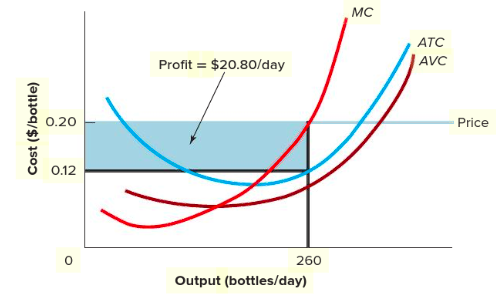
\includegraphics[scale=0.8]{Afsnit/Lektion2/Maksprofit2.png}

Hvis prisen er lavere end de gennemsnitlige total omkostninger vil man have underskud.

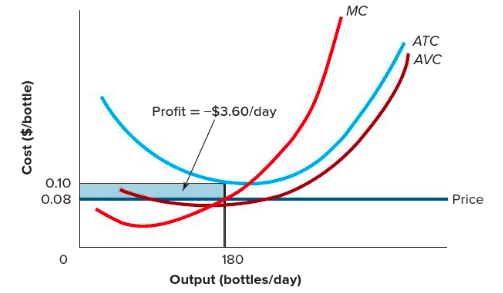
\includegraphics[scale=0.8]{Afsnit/Lektion2/Underskud.png}

\subsubsection{The "law" of supply}
De fuldkommen konkurerende firmaers udbudskurve er kurven for deres marginalomkostninger. For ethvert pris-mængde par langs udbudskurven, er prisen lig sælgerens marginal omkostninger af produktionen. 

\subsection{Determinants of supply revisited}
Hvad kan få udbudskurven til at rykke sig?
\subsubsection{Technology}
Ved teknologisk fremgang bliver det billigere at producere ekstra enheder. Dermed falder marginal omkostningerne og udbudskurven rykkes ned(højre). (sker over tid)
\subsubsection{Input prices}
Ændring i pris af inputs til at producere en varer vil også få udbudskurven til at rykke sig. Hvis lønningerne pludselig stiger, vil marginalomkostningerne stiger og udbudskurven rykker op(venstre). (sker hurtigt)
\subsubsection{The number of suppliers}
Udbudskurven rykker mod højre når antallet af individuelle leverandører vokser. 
\subsubsection{Expectations}
Hvis der er forventninger om at fremtidige priser vil være højere end nutidige priser, holder man på nogle af varerne for at sælge til en højere pris i fremtiden.
\subsubsection{Change in price of other products}
Substitutionseffekten.

\subsubsection{Applying the theory of supply}
Der står ikke noget relevant.

\subsection{Supply and producer surplus}
Som der er noget der hedder forbrugernes overskud, er der også \textbf{sælgers overskud}. Sælgers overskud er forskellen mellem prisen varen sælges for og sælgers mindstepris(reservationspris, marginalomkostning). 

\subsubsection{Calculating producer surplus}
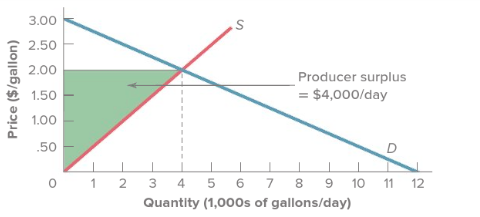
\includegraphics[scale=0.8]{Afsnit/Lektion2/selgeroverskud.png}
Ved ligevægt er overskuddet for sælgerne det stykke der er fra deres mindstepris(kurven) og salgsprisen(trekanten på billedet), og så bare beregn arealet. 


\subsection{Vigtigt fra forelæsningen}

Efterspørgselskurven har negativ hældning pga. loven om aftagende marginalnytte(udover de foregående begrundelser fra lektion 1). Dette gælder da når marginalnytten falder ved at mængden stiger, er folk villige til at betale mindre for det, fordi de får mindre ud af det.

Hvis ens underskud er mindre en ens faste omkostninger skal man bliver ved med at producere da der ville være mere underskud ved ikke at producere end at producere. På lang sigt skal man lukke hvis der er underskud. 

Man vil altid gå efter en produktion der hvor prisen og marginalomkostningerne skærer. Det vil man da det da hvis man sælger mindre udnytter man ikke at man stadig kan sælge mere uden at marginalomkostningerne overstiger ens indtjening per varer. Derudover hvis man er over, vil man for de varer der er over vil man have underskud.

Hvis prisen er under de variable omkostninger er der underskud på kort sigt og de skal lukke. Hvis prisen er under totale omkostninger skal de lukke på lang sigt. 




























